% Matteo Kumar - Leonard Schatt
% Physikalisches Praktikum

% Anhang A

\chapter{Anhang}
\label{chap:anhangA}


\section{Versuchsaufbau}
\label{section:AnhangAufbau} 

\begin{figure}[h]
    \centering
    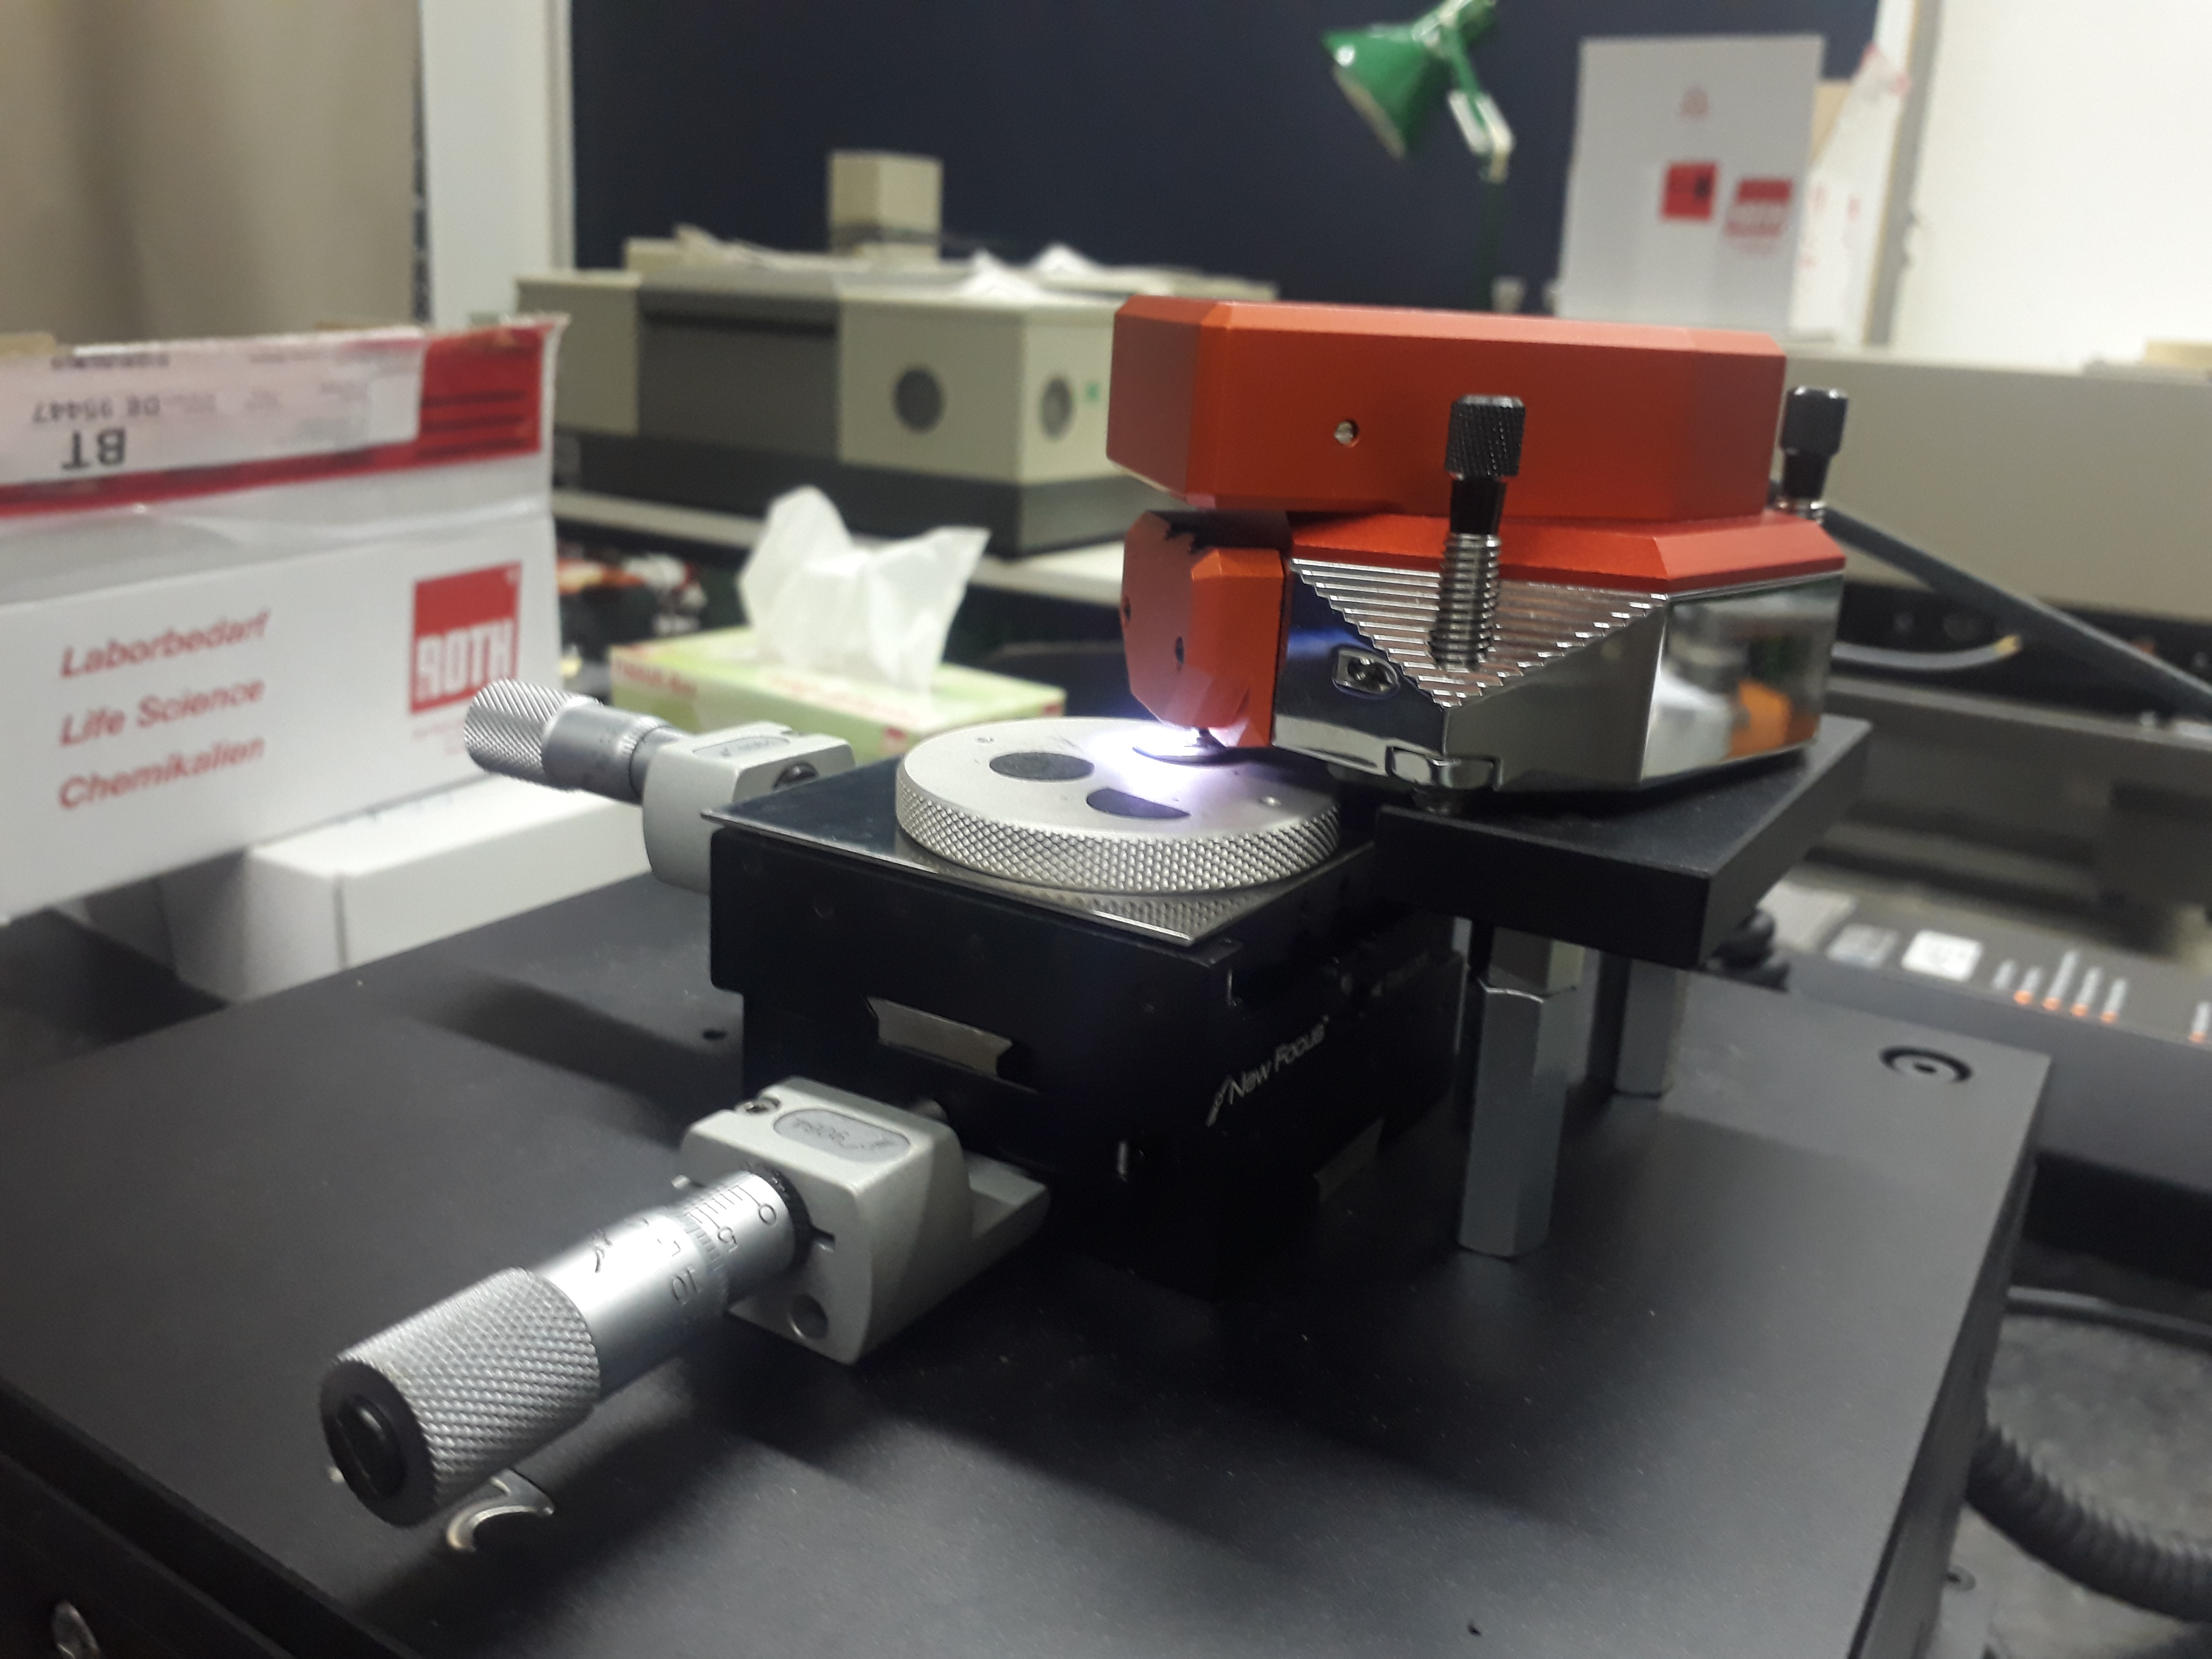
\includegraphics[width = \linewidth]{Bilder/Aufbau/20210920093605.jpg}
    \caption{AFM auf schwingungsdämpfendem Tisch (Nahaufnahme). Schön sichtbar sind die Millimeterschrauben zum Einstellen des Tisches}
\end{figure}

\begin{figure}[h]
    \centering
    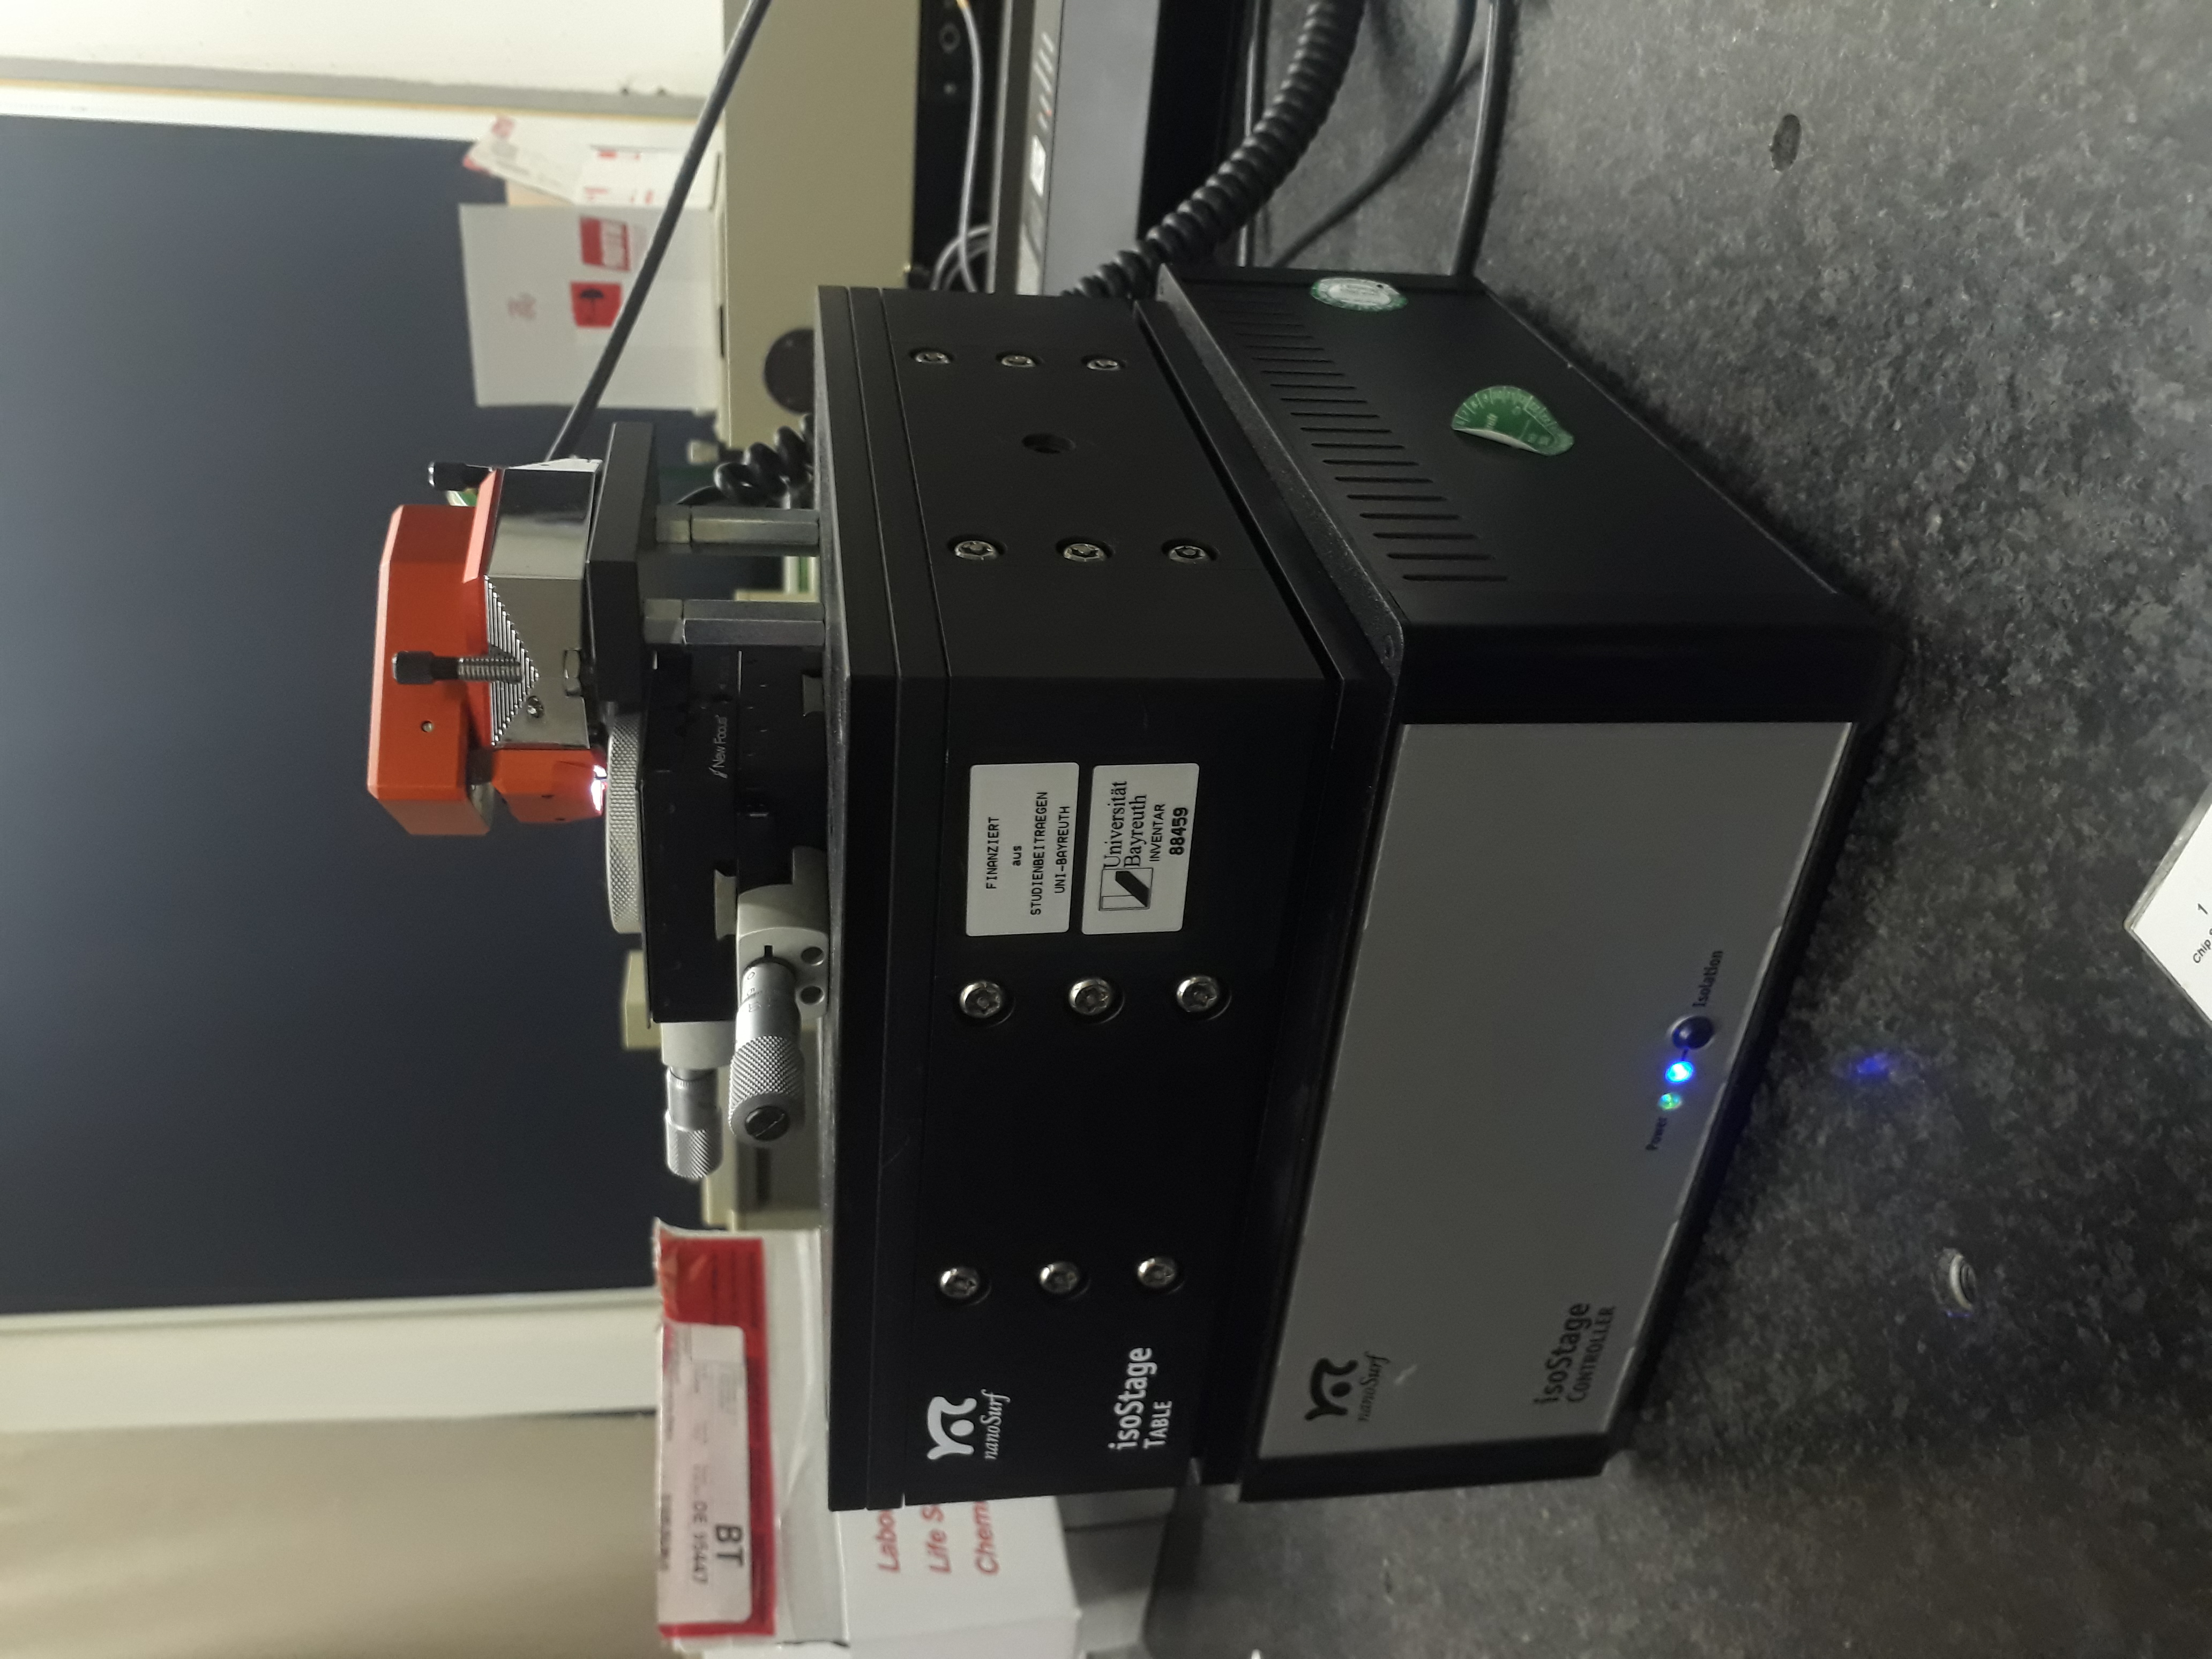
\includegraphics[width = \linewidth, angle = -90]{Bilder/Aufbau/20210920093631.jpg}
    \caption{AFM auf schwingungsdämpfendem Tisch}
\end{figure}

\clearpage



\section{Nanoröhrchen}
\begin{figure}[h]
    \centering
    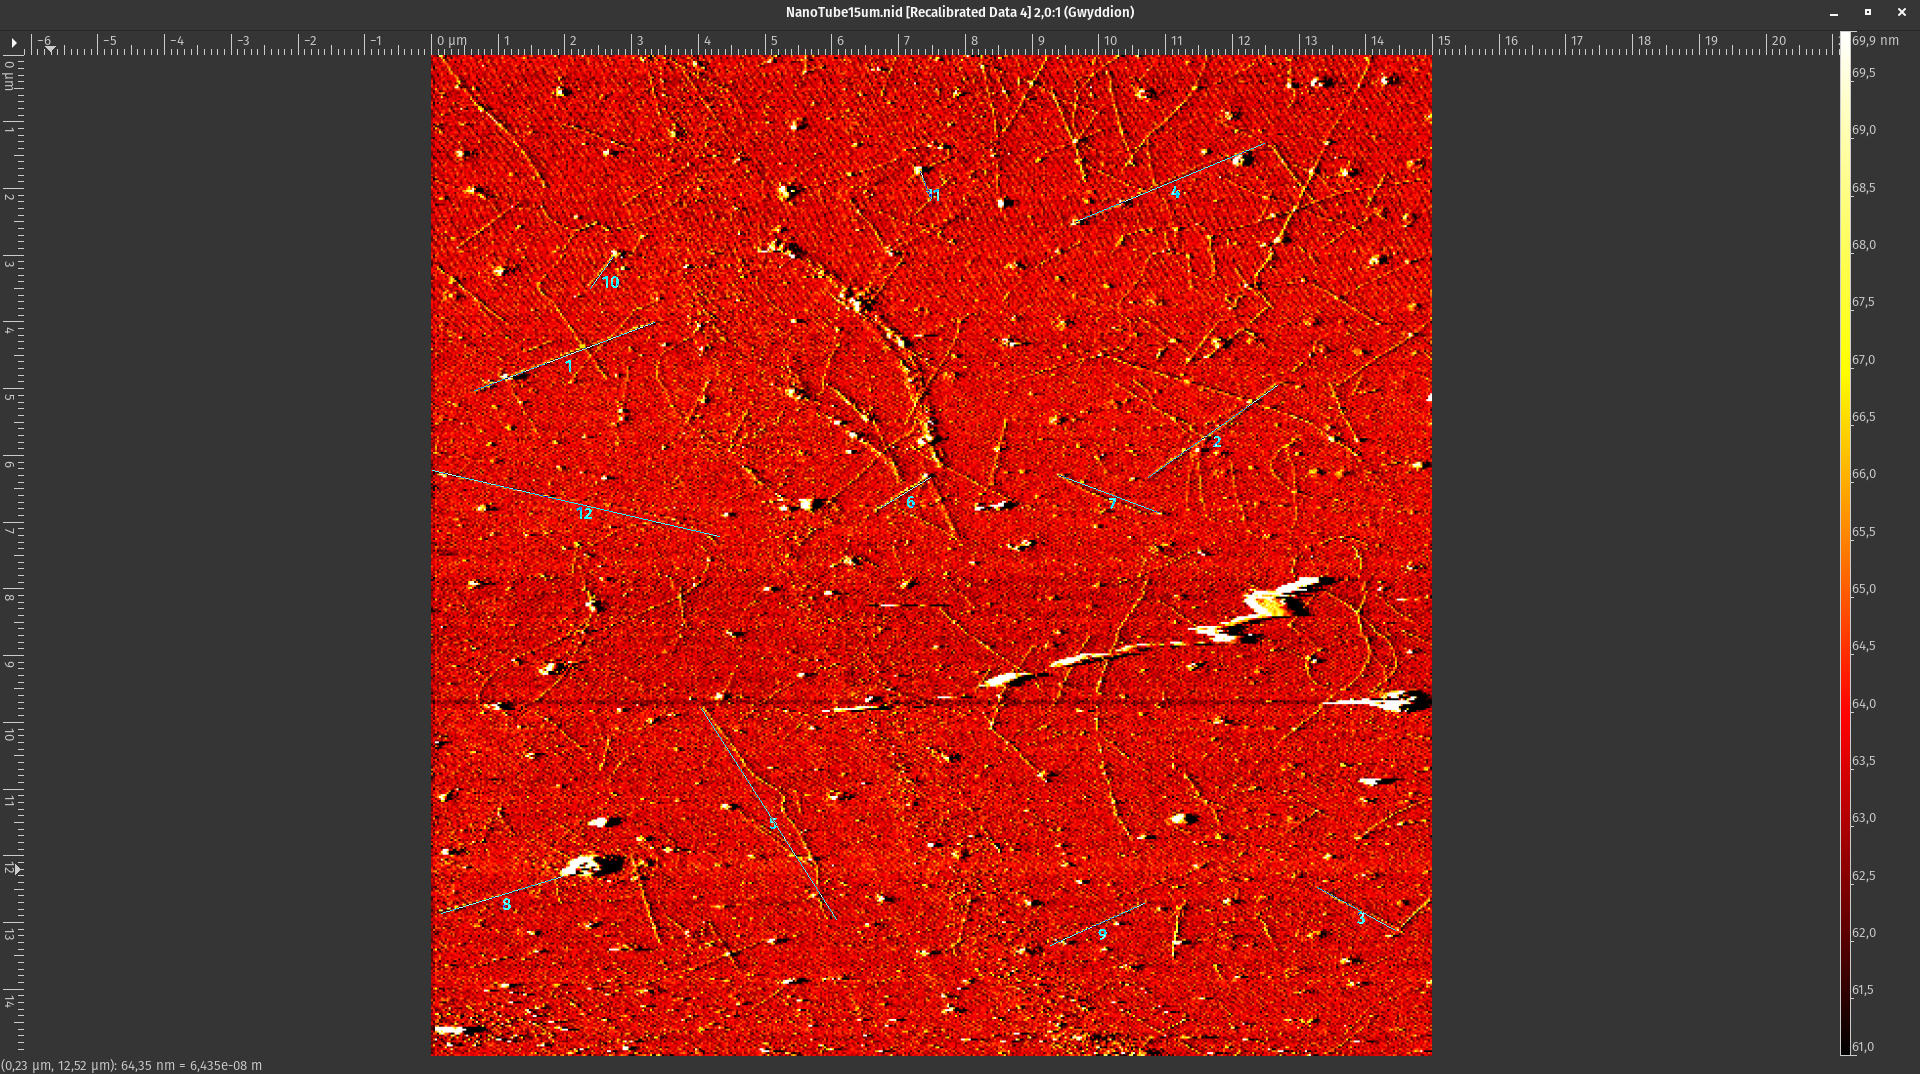
\includegraphics[width = \linewidth]{Bilder/Nanotubes/NanoTube15umLaenge2.png}
    \caption{Nanoröhrchen und die zur Vermessung der Länge gewählten Distanzen}
    \label{Nanotube20Mess}
\end{figure}

\begin{figure}[h]
    \centering
    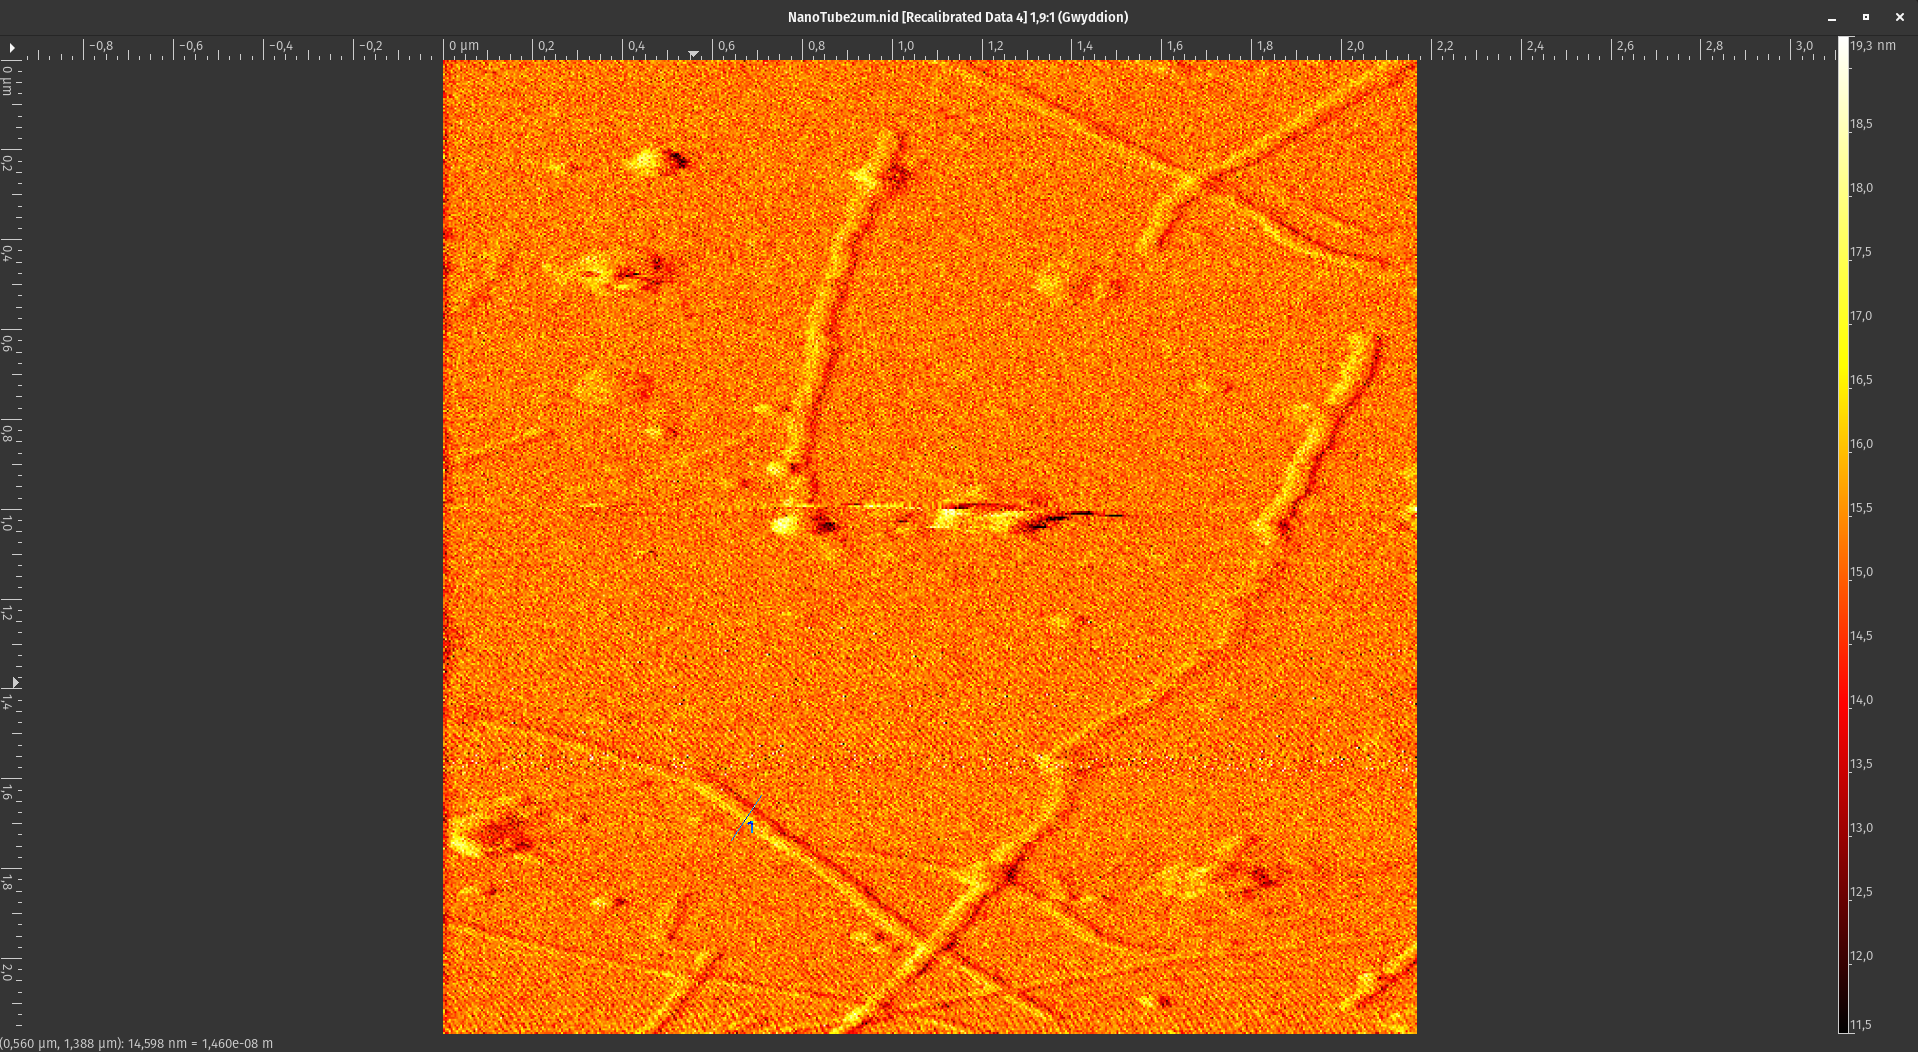
\includegraphics[width = \linewidth]{Bilder/Nanotubes/NanotubesBreiteHoehe2.png}
    \caption{Nanoröhrchen und die zur Vermessung des Radius gewählten Distanzen}
    \label{NanoRadius}
\end{figure}


\clearpage
\section{Gold}

\begin{figure}[h]
    \centering
    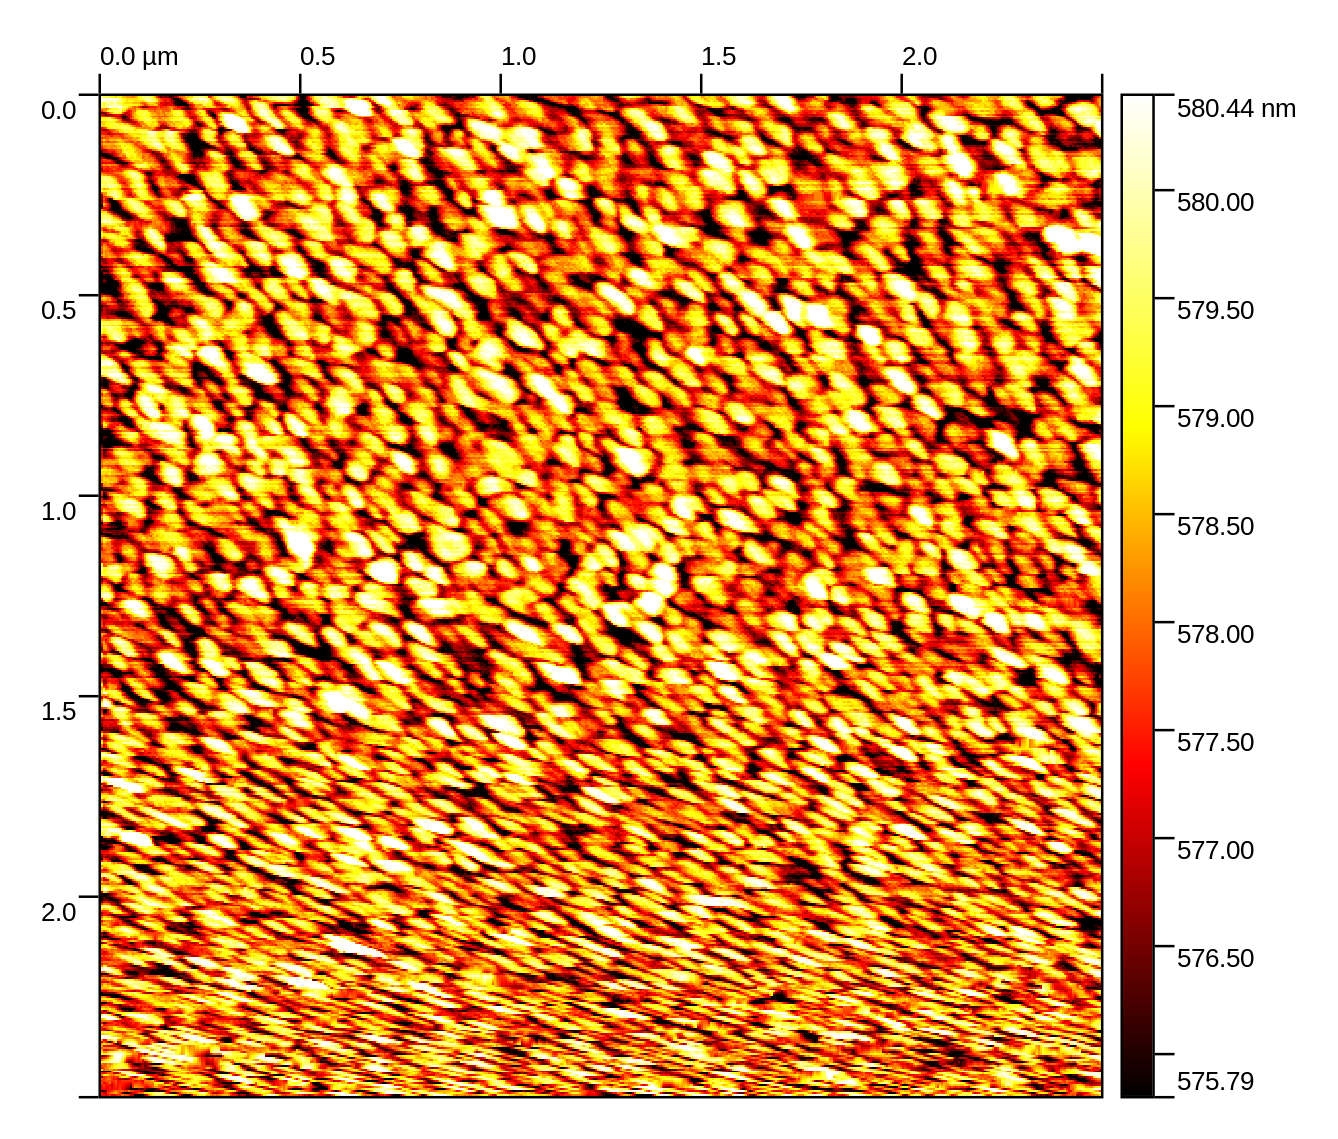
\includegraphics[width = 10cm]{Bilder/Gold/Gold25um.png}
    \caption{Goldprobe unter dem AFM mit einem Ausschnitt von 25x25 $\mu$m}
    \label{Gold1}
\end{figure}


\begin{figure}[h]
    \centering
    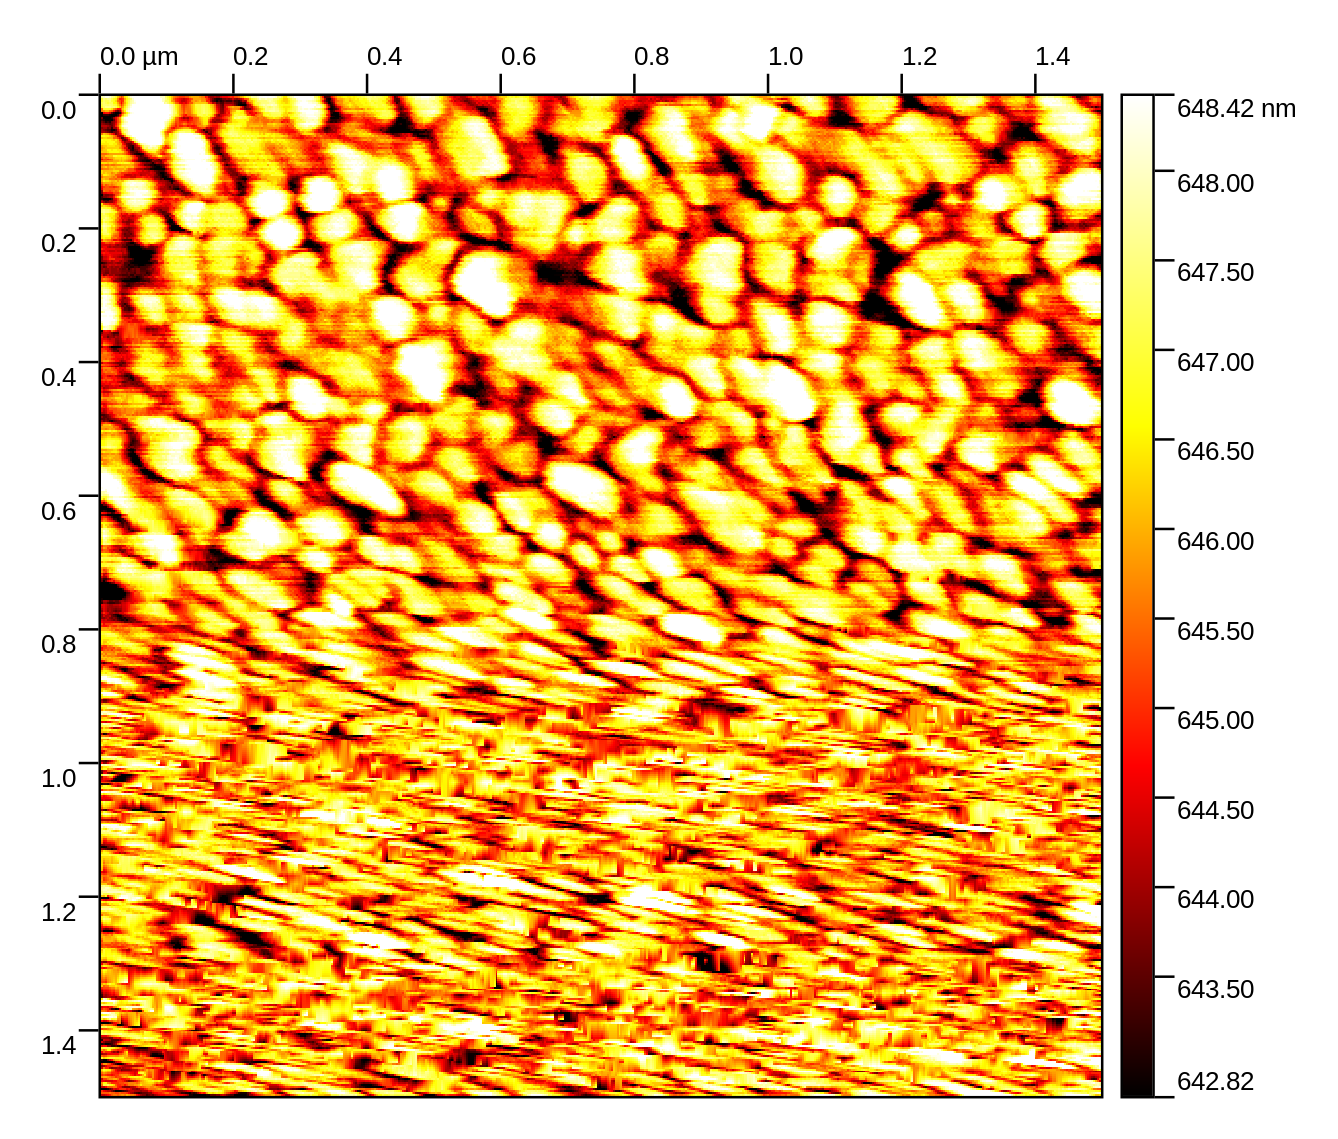
\includegraphics[width = 10cm]{Bilder/Gold/Gold15um.png}
    \caption{Goldprobe unter dem AFM mit einem Ausschnitt von 15x15 $\mu$m}
    \label{Gold2}
\end{figure}



\begin{figure}[h]
    \centering
    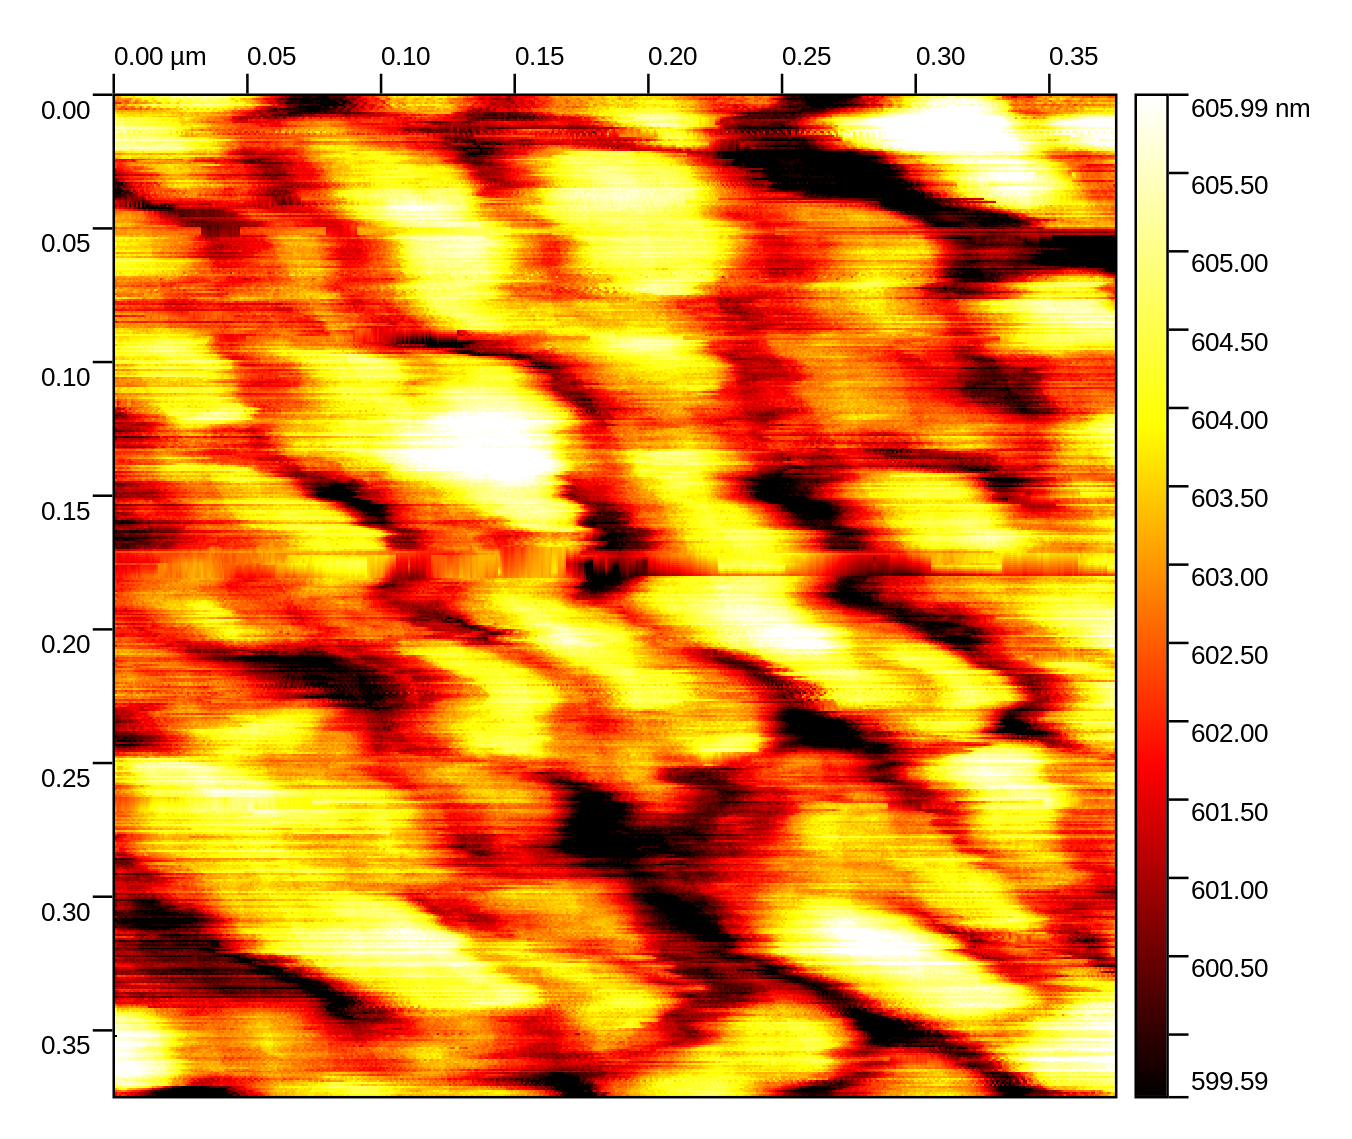
\includegraphics[width = 10cm]{Bilder/Gold/Gold0375um.png}
    \caption{Goldprobe unter dem AFM mit einem Ausschnitt von 0,375x0,375 $\mu$m}
    \label{Gold3}
\end{figure}
